\documentclass[twoside,twocolumn]{article}
\usepackage{blindtext}
\usepackage{graphicx}
\usepackage[sc]{mathpazo}
\usepackage[T1]{fontenc}
\linespread{1.05}
\usepackage{microtype}
\usepackage[english, spanish]{babel}
\usepackage[hmarginratio=1:1,top=32mm,columnsep=20pt]{geometry}
\usepackage[hang, small,labelfont=bf,up,textfont=it,up]{caption}
\usepackage{booktabs}
\usepackage{lettrine}
\usepackage{enumitem}
\setlist[itemize]{noitemsep}
\usepackage{abstract}
\renewcommand{\abstractnamefont}{\normalfont\bfseries} 
\renewcommand{\abstracttextfont}{\normalfont\small\itshape} 
\usepackage{titlesec}
\renewcommand\thesection{\Roman{section}} % 
\renewcommand\thesubsubsection{\roman{subsubsection}} 
\titleformat{\section}[block]{\large\scshape\centering}{\thesection.}{1em}{}
\titleformat{\subsubsection}[block]{\large}{\thesubsubsection.}{1em}{}
\usepackage{fancyhdr} 
\pagestyle{fancy} % All pages have headers and footers
\fancyhead{} % Blank out the default header
\fancyfoot{} % Blank out the default footer
\fancyhead[L]{MLOps} % Custom header text
\fancyhead[R]{Julio 2021} % Custom header text
\fancyfoot[RO,LE]{\thepage} % Custom footer text
\usepackage{titling}
\usepackage{hyperref}

%----------------------------------------------------------------------------------------
%	TILULOS
%----------------------------------------------------------------------------------------

\setlength{\droptitle}{-4\baselineskip}

\pretitle{\begin{center}\Huge\bfseries}
\posttitle{\end{center}} 
\title{MLOps}
\author{Julio Mejia, Randi Paredes, Angel Crispin, Luis Cancino, Derian Herrera}
\date{\today} 
\renewcommand{\maketitlehookd}{
    \selectlanguage{spanish}
    \begin{abstract}
        \noindent Los modelos de machine learning proporcionan insights valiosos al negocio, pero solo si esos modelos pueden acceder a los datos de la organización de forma continua y analizarlos. Las operaciones de machine learning (MLOps por sus siglas en inglés) son el proceso fundamental que lo hace posible.

        Las MLOps son un proceso multifuncional, colaborativo e iterativo que pone en marcha las capacidades de data science. Para ello, las MLOps tratan el machine learning (ML) y otros tipos de modelos como artefactos de software reutilizables. Luego, los modelos se pueden implementar y monitorear continuamente mediante un proceso repetible.
        
        Las MLOps ofrecen una integración continua y una implementación rápida y repetible de modelos. Como tal, ayudan a las empresas a descubrir información e insights valiosos a partir de sus datos con mayor rapidez. Las MLOps también incluyen el monitoreo y la repetición del entrenamiento continuo de modelos en producción para garantizar que funcionen de manera óptima a medida que los datos cambian (evolucionan) con el tiempo.
    \end{abstract}
    \selectlanguage{english}
    \begin{abstract}
        \noindent Machine learning models provide valuable information to the business, but only if those models can continuously access and analyze the organization's data. Machine learning operations (MLOps) are the fundamental process that makes this possible.

        MLOps are a cross-functional, collaborative, and iterative process that puts data science capabilities to work. To do this, MLOps treat machine learning (ML) and other types of models as reusable software artifacts. The models can then be deployed and continuously monitored using a repeatable process.
        
        MLOs offer continuous integration and fast, repeatable model deployment. As such, they help companies discover valuable information and insights from their data faster. MLOps also include continuous monitoring and re-training of models in production to ensure they perform optimally as data changes (evolves) over time.
    \end{abstract}
}

%----------------------------------------------------------------------------------------

\begin{document}

% Print the title
\maketitle

%----------------------------------------------------------------------------------------
%	INTRODUCCION
%----------------------------------------------------------------------------------------

\section{Introduccion}
\lettrine[nindent=0em,lines=3]{L}Los orígenes de MLOps se remontan a 2015 a partir de un artículo titulado "Deuda técnica oculta en sistemas de aprendizaje automático". Y desde entonces, el crecimiento ha sido particularmente fuerte. Tenga en cuenta que se espera que el mercado de soluciones MLOps alcance los \$4 mil millones para 2025..

%----------------------------------------------------------------------------------------
%	DESARROLLO
%----------------------------------------------------------------------------------------

\section{Desarrollo}

\subsection{¿Qué es MLOps?}
\noindent es inteligencia que proporciona un puente entre los científicos de datos y el equipo de producción. Conspira profundamente en la naturaleza y está diseñado para eliminar todos los residuos y hacer que el sistema de aprendizaje automático sea más escalable al proporcionar automatización y producir información altamente consistente del modelo de ML.
MLOps es la idea de combinar la práctica establecida desde hace mucho tiempo de DevOps con el campo emergente del aprendizaje automático. Es la creación de un entorno automatizado para el desarrollo de modelos, el reentrenamiento de modelos, la supervisión de derivas, la automatización de tuberías, el control de calidad y la gobernanza de un modelo en una sola plataforma. Dentro de MLOps existen tres niveles de implementación de Machine Learning:
\begin{itemize}
    \item \textbf{Data}: datos, fase, ingestión, curado, etc.
    \item \textbf{Model}: testing, evaluación de los modelos, empaquetado y como se van a despegar.
    \item \textbf{Code}: el código, donde se ejecuta todo el modelo en sí.
\end{itemize}
\begin{center}
    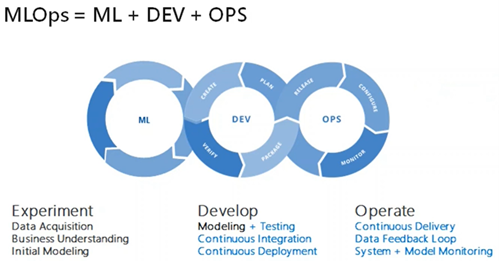
\includegraphics[width=7cm]{./img/img1.png}
\end{center}


\subsection{¿Por qué MLOps?}
\noindent La mayoría de los científicos de datos no son programadores de núcleo duro. Pueden crear el modelo más eficaz para un problema de aprendizaje automático, pero no tienen las habilidades para empaquetar, probar, implementar o mantener este modelo en producción. Se necesita alguien con el conocimiento de bases de datos, API de REST y una colección de otras habilidades de TI para hacerlo. Aquí es donde MLOps entra en escena.
MLOps va más allá del desarrollo y diseño de modelos: también reúne la administración de datos, el desarrollo automatizado de modelos, el reentrenamiento de modelos, la generación de código, el desarrollo continuo y la supervisión del modelo. Al incorporar los principios de DevOps al aprendizaje automático, permite un ciclo de desarrollo más rápido, un mejor control de calidad y la capacidad de responder a los cambiantes requisitos empresariales.

\subsection{Beneficios de MLOps}
Uno de los principales beneficios de las MLOps es que es compatible con tipos de modelos estadísticos, de data science y de aprendizaje automático, entre otros, para ofrecer un valor de negocios rápidamente. Para ello, las MLOps garantizan que los modelos se puedan implementar reiteradamente y monitorear de forma continua. El proceso de MLOps permite lo siguiente:
\begin{itemize}
    \item Implementar más modelos con mayor rapidez con procesos automatizados
    \item Acelerar el tiempo de creación de valor con una rápida entrega de modelos
    \item Optimizar la productividad a través de la colaboración y la reutilización de modelos
    \item Reducir el riesgo de perder tiempo y dinero en modelos que nunca se incorporan a la producción
    \item Monitorear y actualizar continuamente modelos a medida que los datos evolucionan con el tiempo  
\end{itemize}

\subsection{Desafíos de MLOps}
Muchas organizaciones se enfrentan a desafios al trasladar modelos de aprendizaje automatico a entornos de produccion.
En promedio, entre el 60 \% y el 80 \% de los modelos creados con la intencion de implementarlos nunca se llevan a cabo.
Si implementas un modelo que se creo hace un periodo de seis mese a ocho meses, es posible que ese modelo ya este obsoleto.
Las organizaciones que tienen dificultades para integrar las aplicaiones de aprendizaje automatico en las apliaciones de produccion existentes hacen perder tiempo y dinero en proyectos de data science que nunca se incroporan en la produccion.
Las MLOps pueden reducir en gran medida el riesgo de que se produzcan tales fallas y hacer que los modelos se incorporen a la produccion con mayor rapidez, ya que, en definitiva, ahi es donde ofreceran el mayor valor a un negocio.
\subsection{Herramientas}

\begin{itemize}
    \item \textbf{Kubeflow}: Inicialmente, Kubeflow fue iniciado por Google como una plataforma de código abierto para ejecutar Tensorflow usando Kubernetes. Pero ahora se ha expandido para ejecutar marcos multinube y multiarestela que requieren canalizaciones de ML.
    \item \textbf{Algorithmia}: Este famoso marco fue fundado por 2 desarrolladores en Washington DC en 2014. Esta plataforma cuenta actualmente con más de 60000 desarrolladores y más de 4500 algoritmos.
    \item \textbf{Pachyderm}: En esta plataforma, el proceso comienza con el control de versiones de datos combinado con la canalización de datos que da como resultado el linaje de datos y termina con la implementación de modelos de aprendizaje automático. También ofrece control de versiones de los datos para mantener los datos actualizados.
    \item \textbf{MLflow}:Automatiza el desarrollo del modelo y el modelo óptimo se puede seleccionar con mayor facilidad utilizando un servidor de seguimiento.
    \item \textbf{DataRobot}:La mejor parte de esta plataforma es su naturaleza ubicua. Puede acceder a DataRobot en cualquier lugar a través de cualquier dispositivo de múltiples maneras de acuerdo con las necesidades de su negocio.
\end{itemize}
\begin{center}
    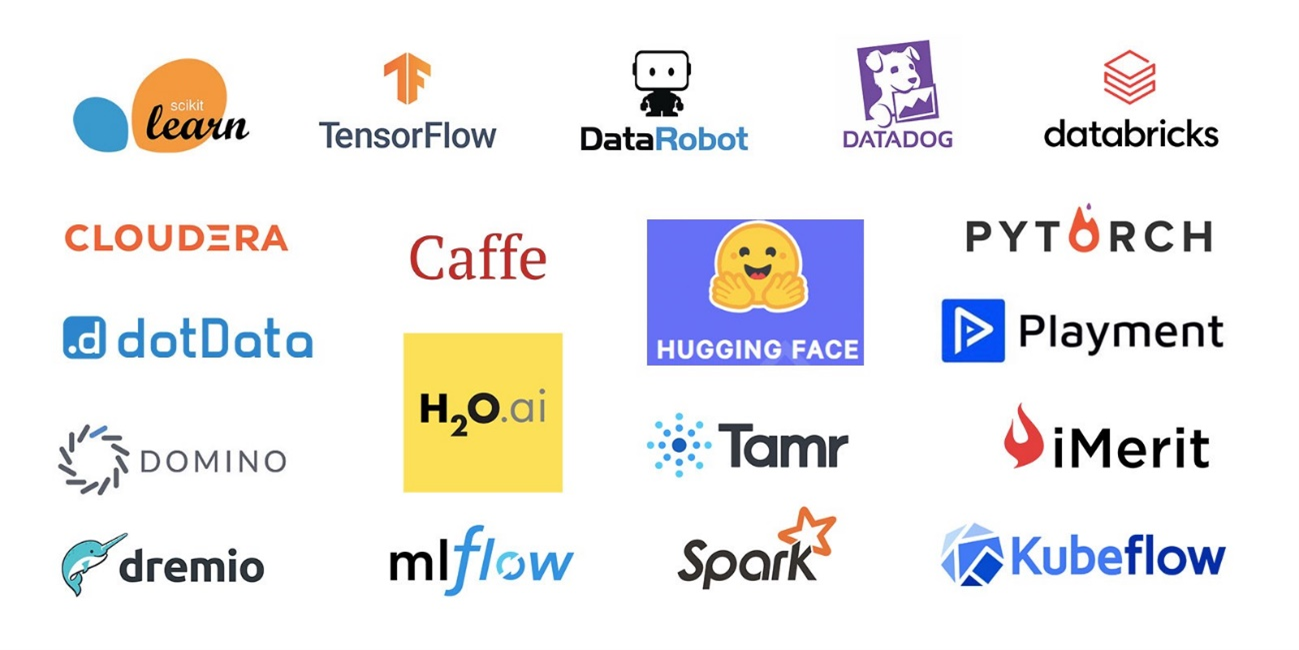
\includegraphics[width=7cm]{./img/img3.png}
\end{center}


\subsection{MLOps frente a DevOps frente a DataOps}
Las MLOps unifican la recopilacion de datos, el procesamiento, el entrenamiento de modelos, la evaluacion, la implementacion y la repeticion del entrenamiento en un solo proceso que los equipos pueden mantener. Esta colaboracion y comunicacion entre DevOps, ITOps, ingenieros de datos, equipos de data science y otros departamentos aportan un entendimiento comun de como se desarrollan y mantienen los modelos de aprendizaje automatico en produccion, de forma similiar a lo que las DevOps hacen por el software. 
Las DevOps se centran en la entrega continua de software y en la automatizacion de la integracion, las pruebas y la implementacion de codigo. No involucran la gestion de datos o analitica. El proceso de MLOps se conforma a partir de las DevOps y se basa en la colaboracion con los equipos de desarrollo para los servicios de implementacion de modelos.

DataOps (operaciones de datos) se encarga de administrar pipelines de datos y automatizar procesos a fin de reducir el tiempo requerido para completar el analisis de datos.

\subsection{Principios de MLOps}
\begin{itemize}
    \item \textbf{Automatización:} Cuyas fases con proceso manual, ML pipeline y CI/CD pipeline.
    \item \textbf{Versionado:} Basado en tres pilares, datos, modelo y código.
    \item \textbf{Testing:} base sobre la que va a funcionar todo el sistema.
    \item \textbf{Monitorización:} Los puntos clave a tener en cuenta son que hay que estar atentos a que no haya cambios en dependencias, hay que asegurar los datos invariantes, el sesgo en predicciones, un modelo “rancio” que no es capaz de responder a la suficiente velocidad, modelo numéricamente estable y degradación del modelo.
    \item \textbf{Reproductividad:} de la ingeniería de características, del entrenamiento del modelo y del despliegue del modelo. Hay que tener cuidado con la recogida de datos, para poder reproducir los resultados.
    \item \textbf{Herramientas:} mlflow, DVC, Kubeflow, ONNX, TensorFlow Extended, Apache Airflow, Cookiecutter, Metaflow, jupyter, PyTorch o Psycaffold.    
\end{itemize}
\begin{center}
    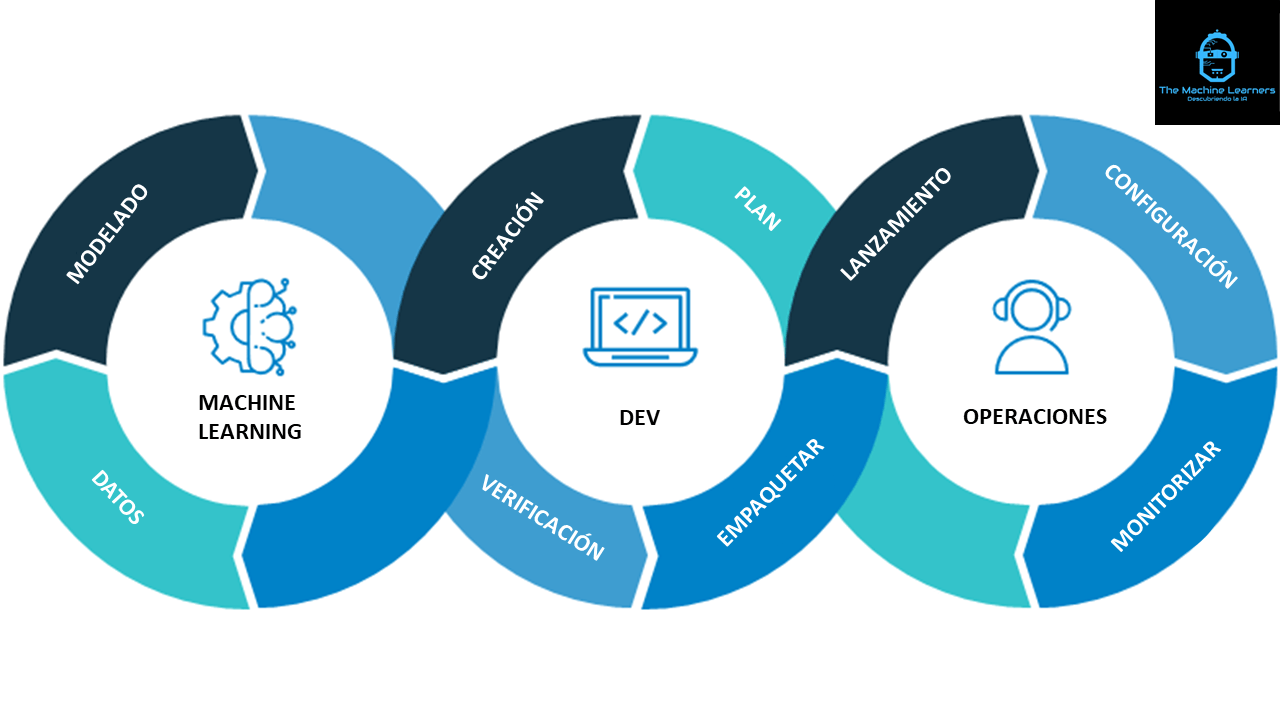
\includegraphics[width=7cm]{./img/img4.png}
\end{center}


%----------------------------------------------------------------------------------------
%	CONCLUSIONES
%----------------------------------------------------------------------------------------

\section{Conclusiones}
\noindent La configuración de MLOps puede ser bastante costosa, pero también ofrece importantes beneficios a las organizaciones que se toman en serio el aprendizaje automático reproducible y la mantenibilidad a largo plazo en un entorno de producción. Los flujos de trabajo de aprendizaje automático automatizados le permiten reciclar y volver a implementar su modelo. La integración continua mantiene el proceso ininterrumpido y mejora continuamente el modelo. El control de versiones de código y datos le permite recrear sus pruebas y revertir los resultados de producción a sus cambios originales. 
A medida que el aprendizaje automático crece como dominio, surgirán nuevos sistemas que facilitarán a su organización la configuración de MLOps. Con el tiempo, MLOps se volverá tan ubicuo e importante como DevOps.

%----------------------------------------------------------------------------------------
%	RECOMENDACIONES
%----------------------------------------------------------------------------------------

\section{Recomendaciones}
\noindent 
Existen varias plataformas MLOps para administrar el ciclo de vida del aprendizaje automático. Asegúrese de tener en cuenta los factores relevantes al seleccionar la plataforma.

%----------------------------------------------------------------------------------------
%	BIBLIOGRAFIA
%----------------------------------------------------------------------------------------

\begin{thebibliography}{99} 
    \bibitem{}
    neptune.ai.(2021) Best End-to-End MLOps Platforms - Leading Machine Learning Platforms That Every Data Scientist Need to Know. Recuperado de 
    \\\texttt{https://n9.cl/a7fnz}
    \bibitem{}
    Alteryx. (2021). ¿Qué son las MLOps y cómo funcionan?. Recuperado de 
    \\\texttt{https://n9.cl/dsg6r}
    \bibitem{}
    Medium. (2020). Introduction to MLOps - ILLUMINATION. Recuperado de 
    \\\texttt{https://n9.cl/hh4or}
    \bibitem{}
    Towards Data Science. (2020). Get started with MLOps. Recuperado de 
    \\\texttt{https://n9.cl/z3fnq}
    \bibitem{}
    Operaciones de Machine Learning (MLOps). (2021).  Recuperado de 
    \\\texttt{https://n9.cl/ha6qz}
\end{thebibliography}
%----------------------------------------------------------------------------------------
\end{document}